\documentclass{beamer}
\beamertemplatenavigationsymbolsempty
\usecolortheme{beaver}
\setbeamertemplate{blocks}[rounded=true, shadow=true]
\setbeamertemplate{footline}[page number]
%
\usepackage[utf8]{inputenc}
\usepackage[english,russian]{babel}
\usepackage{amssymb,amsfonts,amsmath,mathtext}
\usepackage{subfig}
\usepackage[all]{xy} % xy package for diagrams
\usepackage{array}
\usepackage{multicol}% many columns in slide
\usepackage{hyperref}% urls
\usepackage{hhline}%tables

\graphicspath{ {../figures/} }

\begin{document}

\begin{frame}{Anti-Distillation}
Knowledge transfer from a simple model to a complex one.

\begin{columns}[c]
\column{0.6\textwidth}
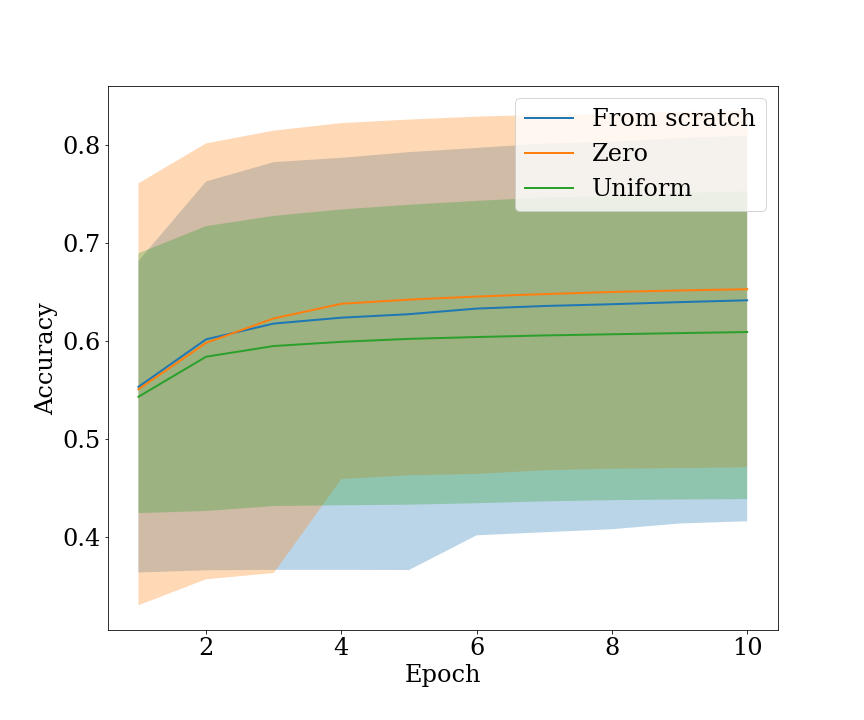
\includegraphics[width=\textwidth]{accuracy.png}
\column{0.5\textwidth}
Weight initialization using the parameters of the pre-trained model.
\end{columns}
% \bigskip
\textbf{Goal}: Adapting the model to more complex data.

\end{frame}

\end{document} 